\documentclass[11pt]{elegantbook}
\usepackage{graphicx}
%\usepackage{float}
\definecolor{structurecolor}{RGB}{40,58,129}
\linespread{1.6}
\setlength{\footskip}{20pt}
\setlength{\parindent}{0pt}
\newcommand{\argmax}{\operatornamewithlimits{argmax}}
\newcommand{\argmin}{\operatornamewithlimits{argmin}}
\elegantnewtheorem{proof}{Proof}{}{Proof}
\elegantnewtheorem{claim}{Claim}{prostyle}{Claim}
\DeclareMathOperator{\col}{col}
\title{Structural Estimation}
\author{Wenxiao Yang}
\institute{Haas School of Business, University of California Berkeley}
\date{2024}
\setcounter{tocdepth}{2}
\extrainfo{All models are wrong, but some are useful.}

\cover{cover.png}

% modify the color in the middle of titlepage
\definecolor{customcolor}{RGB}{32,178,170}
\colorlet{coverlinecolor}{customcolor}
\usepackage{cprotect}


\bibliographystyle{apalike_three}

\begin{document}
\maketitle

\frontmatter
\tableofcontents

\mainmatter

\chapter{Homogenous Products}
How do we estimate demand for a homogenous product?
\section{\cite{working1927statistical}: OLS is not informative with endogeneity}
Demand and Supply for coffee:
\begin{equation}
    \begin{aligned}
        Q^d_t=\alpha_0+\alpha_1 P_t+U_t\\
        Q^s_t=\beta_0+\beta_1 P_t+V_t
    \end{aligned}
    \nonumber
\end{equation}
where $\alpha_1<0$ and $\beta_1>0$. Equilibrium price and quantity are given by
\begin{equation}
    \begin{aligned}
        Q^d_t=Q^s_t \Rightarrow \left\{\begin{matrix}
            P_t=\frac{\beta_0-\alpha_0}{\alpha_1-\beta_1}+\frac{V_t-U_t}{\alpha_1-\beta_1}\\
            Q_t=\frac{\alpha_1\beta_0-\alpha_0\beta_1}{\alpha_1-\beta_1}+\frac{\alpha_1V_t-\beta_1U_t}{\alpha_1-\beta_1}
        \end{matrix}\right.
    \end{aligned}
    \nonumber
\end{equation}
\begin{note}
    Price is a function of both error terms, and we can't use a clever substitution to cancel things out.
\end{note}
We can find that price is positively correlated with demand shift $U_t$ and negatively correlated with supply shift $V_t$.

Consider the OLS estimator: $\hat{\alpha}_1=\hat{\beta}_1=\frac{\textnormal{Cov}(P_t,Q_t)}{\textnormal{Var}(P_t)}$. Since we have
\begin{equation}
    \begin{aligned}
        \left.\begin{matrix}
            \textnormal{Cov}(P_t,Q_t)=\alpha_1\textnormal{Var}(P_t)+\textnormal{Cov}(P_t,U_t)\\
            \textnormal{Cov}(P_t,Q_t)=\beta_1\textnormal{Var}(P_t)+\textnormal{Cov}(P_t,V_t)
        \end{matrix}\right\} \Rightarrow \left\{\begin{matrix}
            \textnormal{Bias}(\alpha_1)=|\hat{\alpha}_1-\alpha_1|=\frac{\textnormal{Cov}(P_t,U_t)}{\textnormal{Var}(P_t)}\\
            \textnormal{Bias}(\beta_1)=|\hat{\beta}_1-\beta_1|=\frac{\textnormal{Cov}(P_t,V_t)}{\textnormal{Var}(P_t)}\\
        \end{matrix}\right.
    \end{aligned}
    \nonumber
\end{equation}
When $\textnormal{Cov}(U_t,V_t)=0$, the OLS estimator can be written as
\begin{equation}
    \begin{aligned}
        \hat{\alpha}_1=\hat{\beta}_1=\frac{\alpha_1\textnormal{Var}(V_t)+\beta_1\textnormal{Var}(U_t)}{\textnormal{Var}(V_t)+\textnormal{Var}(U_t)}
    \end{aligned}
    \nonumber
\end{equation}
More variation in supply $V_t$ gives a better estimate of demand and more variation in demand $U_t$ gives a better estimate of supply.

The OLS is not informative about the economic demand function (or supply function).

To deal with this problem, we need an excluded instrument that shifts one curve without affecting the other. Then, we can use this to form a 2SLS estimate.


\section{\cite{angrist2000interpretation}: IV is limited}
\subsection{Motivation}
What if we don't generality know which kind of heterogeneity we face?

There are four cases that are ranked in increasing complexity:
\begin{enumerate}
    \item Linear system with constant coefficients:
    \begin{equation}
        \begin{aligned}
            q^d_t(p,z,x)=\alpha_0+\alpha_1 p+\alpha_2 z+\alpha_3 x+\epsilon_t\\
            q^s_t(p,z,x)=\beta_0+\beta_1 p+\beta_2 z+\beta_3 x+\eta_t
        \end{aligned}
        \nonumber
    \end{equation}
    \item Linear system with non-constant coefficients:
    \begin{equation}
        \begin{aligned}
            q^d_t(p,z,x)=\alpha_{0t}+\alpha_{1t} p+\alpha_{2t} z+\alpha_{3t} x +\epsilon_t\\
            q^s_t(p,z,x)=\beta_{0t}+\beta_{1t} p+\beta_{2t} z+\beta_{3t} x +\eta_t
        \end{aligned}
        \nonumber
    \end{equation}
    \item Nonlinear system with constant shape (separable):
    \begin{equation}
        \begin{aligned}
            q^d_t(p,z,x)=q^d(p,z,x)+\epsilon_t\\
            q^s_t(p,z,x)=q^s(p,z,x)+\eta_t
        \end{aligned}
        \nonumber
    \end{equation}
    \item Nonlinear system with time-varying shape (non-separable): any forms of $q^d_t(p,z,x)$ and $q^s_t(p,z,x)$.
\end{enumerate}

\subsection{Model}
We assume the regularity conditions (existence of first and second moment and being stationary) and $q^d_t(p,z,x)$, $q^s_t(p,z,x)$ are continuously differentiable in $p$.

\paragraph*{Instrumental Variable}
Assume binary instrument $z_t\in\{0,1\}$ to make things easier. And $z_t\in\{0,1\}$ is a valid instrument in $q^d_t$, i.e., it satisfies
\begin{enumerate}
    \item Exclusion: $q^d_t(p_t,z=1,x_t)=q^d_t(p_t,z=0,x_t)=q^d_t(p_t,x_t)$.
    \item Relevance: $q^s_t(p_t,z=1,x_t)\neq q^s_t(p_t,z=0,x_t)$ for some period $t$.
    \item Independence: $\epsilon_t,\eta_t,z_t$ are mutually independent conditional on $x_t$.
\end{enumerate}

Suppose $z=1$ denote ``stormy at sea'' and $z=0$ denote ``calm at sea''. (Offshore weather makes fishing more difficult but doesn't change onshore demand.)

2SLS can work in linear models,
\begin{equation}
    \begin{aligned}
        \hat{\alpha}_{1,0}=\frac{\widehat{\mathbb{E}_t[q_t|z_t=1]}-\widehat{\mathbb{E}_t[q_t|z_t=0]}}{\widehat{\mathbb{E}_t[p_t|z_t=1]}-\widehat{\mathbb{E}_t[p_t|z_t=0]}}\stackrel{P}{\longrightarrow}\frac{\mathbb{E}_t[q_t|z_t=1]-\mathbb{E}_t[q_t|z_t=0]}{\mathbb{E}_t[p_t|z_t=1]-\mathbb{E}_t[p_t|z_t=0]}:= \alpha_{1,0}
    \end{aligned}
    \nonumber
\end{equation}
but it is not an estimator of a structural parameter in nonlinear models.

\begin{claim}
    Authors make the point that IV estimator identifies something about relationship between $p$ and $q$, without identifying deep structural parameters.
\end{claim}

Some assumptions are needed to interpret the IV estimator.
\begin{assumption}
    \begin{enumerate}
        \item Observed price is market clearing price $q^d_t(p_t)=q^s_t(p_t,z_t)$ for all $t$. (i.e., no friction).
        \item For each value of $z$ and $t$, there is a unique market clearing price, $\tilde{p}(z,t)$, such that
        \begin{equation}
            \begin{aligned}
                q^d_t(\tilde{p}(z,t))=q^s_t(\tilde{p}(z,t),z)
            \end{aligned}
            \nonumber
        \end{equation}
        $\tilde{p}(z,t)$ is the potential price under any counterfactual $(z,t)$.
        \item $\mathbb{E}_t[p_t|z_t=1]\neq\mathbb{E}_t[p_t|z_t=0]$
        \item $\tilde{p}(z,t)$ is weakly increasing in $z$.
    \end{enumerate}
\end{assumption}


\begin{lemma}
    The numerator of $\alpha_{1,0}$ can be given by
    \begin{equation}
        \begin{aligned}
            \mathbb{E}_t[q_t|z_t=1]-\mathbb{E}_t[q_t|z_t=0]=\mathbb{E}_t\left[\int_{\tilde{p}(0,t)}^{\tilde{p}(1,t)}\frac{\partial q^d_t(s)}{\partial s}ds\right]
        \end{aligned}
        \nonumber
    \end{equation}
\end{lemma}

\begin{theorem}
    Based on this lemma, the IV estimator equals to
    \begin{equation}
        \begin{aligned}
            \alpha_{1,0}&=\frac{\mathbb{E}_t\left[\int_{\tilde{p}(0,t)}^{\tilde{p}(1,t)}\frac{\partial q^d_t(s)}{\partial s}ds\right]}{\mathbb{E}_t\tilde{p}(1,t)-\mathbb{E}_t\tilde{p}(0,t)}\\
            &\rightarrow \int_0^\infty \mathbb{E}_t\left[\frac{\partial q^d_t(s)}{\partial s}\mid s\in[\tilde{p}(0,t),\tilde{p}(1,t)]\right]\omega(s)ds
        \end{aligned}
        \nonumber
    \end{equation}
    where $\omega(s)$ is the weight that is not a function of $t$, but it is largest for prices most likely to fall in $[\tilde{p}(0,t),\tilde{p}(1,t)]$.
\end{theorem}
\begin{note}
    \begin{enumerate}
        \item $\alpha_{1,0}$ only provides information about demand curve in range of potential price variation induced by the instrument.
        \item  For different instruments $z$, $\alpha_{1,0}$ has a different interpretation like the LATE does. (Different from the linear model where anything works!).
    \end{enumerate}
\end{note}




















\chapter{Random Utility Models}
\section{Gumbel Distribution}
\begin{definition}[Gumbel Distribution]
    \textbf{Gumbel distribution} is also called \textbf{type-I generalized extreme value distribution}, denoted by $\textnormal{Gumbel}(\mu,\beta)$. The $\mu$ is the location and $\beta>0$ is the scale.

    Its cdf is
    \begin{equation}
        \begin{aligned}
            F(x,\mu,\beta)=e^{-e^{-(x-\mu)/\beta}},
        \end{aligned}
        \nonumber
    \end{equation}
    and its pdf is
    \begin{equation}
        \begin{aligned}
            f(x,\mu,\beta)=\frac{1}{\beta} e^{-(z+e^{-z})}, \textnormal{ where }z=\frac{x-\mu}{\beta}
        \end{aligned}
        \nonumber
    \end{equation}
\end{definition}
\begin{lemma}[Properties of Gumbel Distribution]
    The properties of Gumbel distribution are given as follows.
    \begin{enumerate}
        \item The mean is $\mathbb{E}[X]=\mu+\gamma\beta$, where $\gamma$ is the Euler-Mascheroni constant.
        \item The median is $\mu-\beta\ln (\ln 2)$;
        \item The variance is $\frac{\pi^2}{6}\beta^2$;
        \item If $G_1,...,G_k$ are i.i.d. Gumbel random variables with parameters $(\mu,\beta)$, its maximum is also a Gumbel random variable,
        \begin{equation}
            \begin{aligned}
                \max\{G_1,...,G_k\}\sim \textnormal{Gumbel}(\mu+\beta\ln k,\beta).
            \end{aligned}
            \nonumber
        \end{equation}
        Then, $\mathbb{E}[\max\{G_1,...,G_k\}]=\mu+\beta\ln k + \gamma\beta$.
    \end{enumerate}
\end{lemma}
\begin{lemma}\label{lemma:max_gumbel}
    Suppose $g_1,...,g_n$ be independent samples of $\textnormal{Gumbel}(0,1)$. Then,
    \begin{enumerate}
        \item $\argmax_i(g_i + \delta_i)\sim \textnormal{Categorical}\left(\frac{e^{\delta_j}}{\sum_{i}e^{\delta_i}}\right)_j$.
        \item $\max_{i}(g_i + \delta_i) \sim \textnormal{Gumbel}\left(\log\left(\sum_{i}e^{\delta_i}\right),1\right)$.
        \item $\mathbb{E}[\max_{i}(g_i + \delta_i)]=\log\left(\sum_{i}e^{\delta_i}\right)+\gamma$.
    \end{enumerate}
\end{lemma}
\section{Random Utility Models}
Content is based on \cite{berry2021foundations}.\\
Let $j=1,...,J_i$ index the ``inside goods'' available to consumer $i$ while $j=0$ denotes the outside good. A consumer's choice set is characterized by $J_i$ and a set $\chi_i$, which may include
\begin{enumerate}[$\circ$]
    \item observed characteristics of consumer $i$,
    \item observed characteristics of goods (including prices),
    \item observed characteristics of the local market,
    \item and characteristics of the market or goods that are unobserved to the researcher.
\end{enumerate}
Each consumer $i$ has a (conditional indirect) utility $u_{ij}$ for good $j$. Consumer knows her utilities for all goods and chooses the good with the highest utility.

In this model, the heterogeneity of consumer preferences is modeled by random utilities:
\begin{definition}[Random Utility Model]
    Given the choice set $(J_i, \chi_i)$, each consumer's utility vector $(u_{ij})_{j=0,1,...,J_i}$ is an independent draw from a joint distribution $F_u(\cdot\mid J_i, \chi_i)$.
\end{definition}
Since only the ordinal ranking of goods matters for a consumer's behavior, we can normalize the location and scale of each consumer's utility vector without loss of generality. We assume that ``ties'' ($u_{ij}=u_{ik}$ for some $j\neq k$) occur with probability zero in the distribution $F_u(\cdot\mid J_i, \chi_i)$. Then, we can represent consumer $i$'s choice with the vector $(q_{i1},...,q_{iJ_i})$, where
\begin{equation}
    \begin{aligned}
        q_{ij}=\mathbf{1}\{u_{ij}\geq u_{ik},\forall k\}
    \end{aligned}
    \nonumber
\end{equation}
The consumer-specific choice probabilities are then given by
\begin{equation}
    \begin{aligned}
        s_{ij}:=\mathbb{E}[q_{ij}\mid J_i,\chi_i]=\int_{\mathcal{A}_{ij}}d F_u\left(u_{i0},...,u_{iJ_i}\mid J_i, \chi_i\right)
    \end{aligned}
    \nonumber
\end{equation}
where $\mathcal{A}_{ij}=\{(u_{i0},...,u_{iJ_i})\in\mathbb{R}^{J_i+1}\mid u_{ij}\geq u_{ik},\forall k\}$.



\section{The Canonical Model}
\begin{definition}[Canonical Model: Independence of Irrelevant Alternatives (IIA)]
    Discrete choice demand models are frequently formulated using a parametric random utility specification such as
    \begin{equation}
        \begin{aligned}
            u_{ijt}=x_{jt}\beta_{it}-\alpha_{it}p_{jt}+\xi_{jt}+\epsilon_{ijt}
        \end{aligned}
        \nonumber
    \end{equation}
    for $j>0$, with $u_{i0t}=\epsilon_{i0t}$.
\end{definition}

The notion of a “market” $t$ allows a precise characterization of the endogeneity problems inherent to demand estimation (In practice, markets are typically defined by natural combinations of time and geography). Let $\mathcal{J}_t$ denote the set of products (inside goods) available to consumers in market $t$, and let $J_t=|\mathcal{J}_t|$.

Let $x_t=(x_{1t},...,x_{J_t,t}), p_t=(p_{1t},...,p_{J_t,t}), \xi_t=(\xi_{1t},..., \xi_{J_t,t})$, and $\chi_t=(x_t,p_t,\xi_t)$.

\begin{enumerate}
    \item $p_{jt}$ represents the price of good $j$ in market $t$, while $x_{jt}\in \mathbb{R}^K$ represents other observable characteristics of good $j$ in the market.
    \item $\xi_{jt}$ is \textit{ a demand shock}, an unobserved factor associated with good $j$ and market $t$.
    \subitem $\circ$ ($\xi_{jt}$ can represent any combination of latent taste variation and latent product characteristics common to consumers in market $t$. For example, a high value of $\xi_{jt}$ may simply indicate that consumers in market $t$ have a high mean taste for good $j$.)
    \subitem $\circ$ ($\xi_{jt}$ is correlated with $p_{jt}$ and $x_{jt}$ by the endogeneity of prices and additional characteristics.)
    \subitem $\circ$ ($\xi_{jt}$ is not a characteristic, i.e., $\mathbb{E}[\xi_{jt}\mid x_{jt}]=0$.)
    \item $\epsilon_{ijt}$ is the \textit{utility shock}. It is most often specified as an i.i.d. draw from a standard type-1 extreme value distribution, yielding a \textit{mixed multinomial logit model}.
    \subitem $\circ$ Choice probabilities in the population reflect a mixture of the choice probabilities conditional on each possible combination of ($\alpha_{it},\beta_{it}$). In this case, the choice probabilities in the population (i.e., the market shares) are given by
    \begin{equation}
        \begin{aligned}
            s_{jt}=\int \frac{\exp(x_{jt}\beta_{it}-\alpha_{it}p_{jt}+\xi_{jt})}{\sum_{k=0}^{J_t}\exp(x_{kt}\beta_{it}-\alpha_{it}p_{kt}+\xi_{kt})}d F(\alpha_{it},\beta_{it};t)
        \end{aligned}
        \label{eq:mixed_multinomial_logit}
    \end{equation}
    where the latent taste parameters $\alpha_{it}$ and $\beta_{it}$ are often referred to as ``random coefficients,'' and $F(\cdot;t)$ denotes their joint distribution in market $t$.
    \subitem $\circ$ Alternatively, a normal distribution will yield a mixed multinomial probit.
    \item The joint distribution $F(\cdot;t)$ is commonly specified as follows.
    \begin{enumerate}
        \item Each component $k$ of the random coefficient vector $\beta_{it}$ typically specified takes the form
        \begin{equation}
            \begin{aligned}
                \beta_{it}^{(k)}=\beta_{0}^{(k)}+\beta_{v}^{(k)}v_{it}^{(k)}+\sum_{l=1}^L\beta_{d}^{(l,k)}d_{ilt}
            \end{aligned}
            \label{eq:beta_it}
        \end{equation}
        Remind that the $\beta_{it}^{(k)}$ contributes as $x_{jt}^{(k)}\beta_{it}^{(k)}$.
        \begin{enumerate}
            \item The $\beta_{0}^{(k)}$ is a parameter shifting \underline{all} consumers' tastes for additional characteristics $x_{jt}^{(k)}$.
            \item Each $d_{ilt}$ represents a \textit{characteristic} (e.g., demographic measure) of individual $i$; the $\beta_{d}^{(l,k)}$ governs the extent of variation in tastes for $x_{jt}^{(k)}$ with different values of $d_{ilt}$.
            \item Each $v_{it}^{(k)}$ represents a \textit{taste shock}, which is a random variable with a pre-specified distribution (e.g., a standard normal); the $\beta_{v}^{(k)}$ governs the extent of variation in tastes for $x_{jt}^{(k)}$ with different values of $v_{it}^{(k)}$.
        \end{enumerate}
        \item A typical specification of $\alpha_{it}$ takes the form
        \begin{equation}
            \begin{aligned}
                \ln(\alpha_{it})=\alpha_0+\alpha_y y_{it}+\alpha_v v_{it}^{(0)}
            \end{aligned}
            \label{eq:alpha_it}
        \end{equation}
        where $y_{it}$ represents consumer-specific measures such as income that are posited to affect price sensitivity. The variables included in $y_{it}$ might overlap partially or entirely with $d_{it}$.
    \end{enumerate}
\end{enumerate}



\section{Market-Level Data}
We typically observe key data at the market level:
\begin{enumerate}
    \item $J_t$: the number of goods available to consumers in each market $t$;
    \item $p_t,x_t$: prices and additional characteristics of goods in each market $t$;
    \item $\tilde{s}_{jt}$: observed market shares, typically measured by $\tilde{s}_{jt}:=\frac{\textnormal{total quantity of good $j$ sold in market $t$}}{\textnormal{total number of consumers in market $t$}}$.
    \item \textit{Distributions of $(d_{it},y_{it})$}: distribution of consumer characteristics in each market.
    \item Additional variables $w_t$ that might serve as appropriate instruments.
\end{enumerate}


\section{\cite{mcfadden1972conditional,mcfadden1981econometric}}
\subsection{Elasticity of Multinomial Logit Model}
Consider the multinomial logit model with $u_{ij}=\beta x_j+\epsilon_{ij}$, the market shares are given by
\begin{equation}
    \begin{aligned}
        s_{ij}=\frac{\exp\left(\beta x_j\right)}{\sum_{k=0}^{J}\exp\left(\beta x_k\right)}
    \end{aligned}
    \nonumber
\end{equation}
where
\begin{equation}
    \begin{aligned}
        \frac{\partial s_{ij}}{\partial x_j}%=\frac{\beta\exp\left(\beta x_j\right)\left(\sum_{k=0}^{J}\exp\left(\beta x_k\right)-\exp\left(\beta x_j\right)\right)}{\left(\sum_{k=0}^{J}\exp\left(\beta x_k\right)\right)^2}
        =\beta s_{ij}(1-s_{ij});\quad
        \frac{\partial s_{ij}}{\partial x_k}=-\beta s_{ij}s_{ik}
    \end{aligned}
    \nonumber
\end{equation}
Then, the \textbf{elasticity} and \textbf{cross elasticity} are given by
\begin{equation}
    \begin{aligned}
        \frac{\partial \log s_{ij}}{\partial \log x_j}=\beta x_j (1-s_{ij});\quad \frac{\partial \log s_{ij}}{\partial \log x_k}=-\beta x_k s_{ik}
    \end{aligned}
    \nonumber
\end{equation}

By the Lemma \ref{lemma:max_gumbel}, the \textbf{expected utility of the consumer} $i$ is $$\mathbb{E}[\max_{j\in\{0,1...,J\}} u_{ij}]=\log\left(\sum_{k=0}^{J}\exp\left(\beta x_k\right)\right)+\gamma$$

The \textbf{diversion ratio} is the probability that consumer $i$, who leaves product $j$ after a decrease in $x_j$, switches to product $k$:
\begin{equation}
    \begin{aligned}
        D_{ijk}=\bigg|\frac{\frac{\partial s_{ik}}{\partial x_j}}{\frac{\partial s_{ij}}{\partial x_j}}\bigg|=\frac{s_{ik}}{1-s_{ij}}
    \end{aligned}
    \nonumber
\end{equation}


\subsection{Nested Logit Model}
A traditional relaxation of IIA is the Nested Logit Model, which is usually presented as two sequential decisions:
\begin{figure}[htbp]
    \centering
    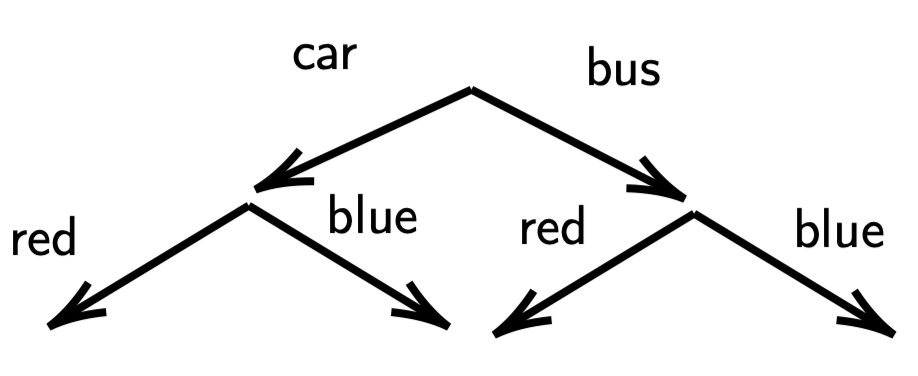
\includegraphics[scale=0.3]{Nest.png}
    \caption{Nested Logit Model}
    \label{}
\end{figure}
The utility of $i$ from product $j$ is given by
\begin{equation}
    \begin{aligned}
        u_{ij}=\delta_{ij}+\zeta_{ig}+(1-\rho)\epsilon_{ij}
    \end{aligned}
    \nonumber
\end{equation}
where $\delta_{ij}$ is the utility we want to estimate in multinomial logit, $\zeta_{ig}$ is a common preferences over all products that belong to the nest $g$.

$\rho$ is often interpreted as a within-nest correlation of preferences. If $\rho=0$, we are in the simple logit case.

\begin{note}
    IIA still holds within each nest and also between the nests.
\end{note}

The distribution of $\zeta_{ig}+(1-\rho)\epsilon_{ij}$ is a special case of a GEV distribution such that
\begin{equation}
    \begin{aligned}
        p_{ij}=\frac{\exp\left(\frac{\delta_{ij}}{1-\rho}\right)\left(\sum_{k\in g}\exp\left(\frac{\delta_{ik}}{1-\rho}\right)\right)^{-\rho}}{\sum_{h \in G}\left(\sum_{k\in h}\exp\left(\frac{\delta_{ik}}{1-\rho}\right)\right)^{1-\rho}}
    \end{aligned}
    \nonumber
\end{equation}
where $G$ is the set of nests. This probability can be decomposed into two probabilities:
\begin{equation}
    \begin{aligned}
        p_{ij}=\underbrace{\frac{\exp\left(\frac{\delta_{ij}}{1-\rho}\right)}{\sum_{k\in g}\exp\left(\frac{\delta_{ik}}{1-\rho}\right)}}_{p_{ij|g}}\underbrace{\frac{\exp\left((1-\rho)\mathbb{E}[\max_{j\in g}u_{ij}]\right)}{\sum_{h \in G}\exp\left((1-\rho)\mathbb{E}[\max_{j\in h}u_{ij}]\right)}}_{p_{ig}}
    \end{aligned}
    \nonumber
\end{equation}
where $\mathbb{E}[\max_{j\in h}u_{ij}]=\log\left(\sum_{k\in h}\exp\left(\frac{\delta_{ik}}{1-\rho}\right)\right)+\gamma$.

\section{\cite{berry1994estimating}: IV-based estimation with unobserved demand shock}
Consider the case without random coefficients, i.e., $(\alpha,\beta)$ are common across all $i$:
\begin{equation}
    \begin{aligned}
        u_{ijt}=\underbrace{x_{jt}\beta-\alpha p_{jt}+\xi_{jt}}_{:=\delta_{jt}}+\epsilon_{ijt}
    \end{aligned}
    \nonumber
\end{equation}
In MNL case, the choice probabilities in the population are given by
\begin{equation}
    \begin{aligned}
        s_{jt}=\frac{\exp(x_{jt}\beta-\alpha p_{jt}+\xi_{jt})}{1+\sum_{k=1}^{J_t}\exp(x_{kt}\beta-\alpha p_{kt}+\xi_{kt})}=\frac{\exp(\delta_{jt})}{1+\sum_{k=1}^{J_t}\exp(\delta_{kt})}:=\hat{s}_{jt}(\delta_{1t},...,\delta_{J_tt})
    \end{aligned}
    \label{eq:s_jt}
\end{equation}
for $j=1,...,J_t$ and $s_{0t}=\frac{1}{1+\sum_{k=1}^{J_t}\exp(x_{kt}\beta-\alpha p_{kt}+\xi_{kt})}$.

\begin{note}
    We cannot do \textbf{nonlinear least squares, i.e.}
    \begin{equation}
        \begin{aligned}
            \min_{\alpha,\beta} \sum_{j=1}^{J_t}\left(\tilde{s}_{jt}-\frac{\exp(x_{jt}\beta-\alpha p_{jt}+\xi_{jt})}{1+\sum_{k=1}^{J_t}\exp(x_{kt}\beta-\alpha p_{kt}+\xi_{kt})}\right)^2
        \end{aligned}
        \nonumber
    \end{equation}
    because we need to know the $x_{jt}$ in order to estimate $\alpha$ and $\beta$.
\end{note}

\subsection{Welfare}
By the Lemma \ref{lemma:max_gumbel}, the consumer's welfare based on utility is given as
\begin{equation}
    \begin{aligned}
        \mathbb{E}[\max_{j} u_{ijt}]=\log\left(1+\sum_{j=1}^{J}\exp(\delta_{jt})\right)+\gamma.
    \end{aligned}
    \nonumber
\end{equation}
Suppose the $\delta_{jt}$ change to $\delta'_{jt}$. Then the welfare change in utility is
\begin{equation}
    \begin{aligned}
        \log\left(1+\sum_{j=1}^{J}\exp(\delta'_{jt})\right)-\log\left(1+\sum_{j=1}^{J}\exp(\delta_{jt})\right),
    \end{aligned}
    \nonumber
\end{equation}
and the welfare change in dollars is
\begin{equation}
    \begin{aligned}
        \Delta CW=\frac{1}{\alpha}\left[\log\left(1+\sum_{j=1}^{J}\exp(\delta'_{jt})\right)-\log\left(1+\sum_{j=1}^{J}\exp(\delta_{jt})\right)\right].
    \end{aligned}
    \nonumber
\end{equation}






\subsection{Inversion}
\cite{berry1994estimating} suggests an IV-based estimation with unobserved demand shock:

Assume there exist instruments $z_{jt}$ such that $\mathbb{E}[\xi_{jt}z_{jt}]=0$. The corresponding moment condition is
\begin{equation}
    \begin{aligned}
        \frac{1}{J_t}\sum_{j=1}^{J_t}\xi_{jt}z_{jt}=\frac{1}{J_t}\sum_{j=1}^{J_t}\left(\delta_{jt}-x_{jt}\beta+\alpha p_{jt}\right)z_{jt} \stackrel{J \rightarrow \infty}{\longrightarrow} 0
    \end{aligned}
    \label{eq:iv_moment}
    \tag{Sample Moment}
\end{equation}
which converges to zero at the true value of $\alpha$ and $\beta$. We want to estimate $\alpha$ and $\beta$ by minimizing the sample moment. However, we do not know $\delta_{jt}$.
\begin{definition}
    \cite{berry1994estimating} suggests a two-step approach
    \begin{enumerate}
        \item \textbf{Inversion}: By equating the data $\tilde{s}_{jt}$ and the choice probabilities $\hat{s}_{jt}(\delta_{1t},...,\delta_{Jt})$, we have a system of $J$ nonlinear equations:
        \begin{equation}
            \begin{aligned}
                \left\{\begin{matrix}
                    \tilde{s}_{1t}&=\hat{s}_{1t}(\delta_{1t},...,\delta_{J_tt})\\
                    \vdots&\vdots\\
                    \tilde{s}_{J_tt}&=\hat{s}_{J_tt}(\delta_{1t},...,\delta_{J_tt})\\
                \end{matrix}\right.
            \end{aligned}
            \nonumber
        \end{equation}
        Then, we can ``inverse'' this system of equations to solve for $\delta_{1t},...,\delta_{J_tt}$ as a function of $\tilde{s}_{1t},...,\tilde{s}_{J_tt}$:
        \begin{equation}
            \begin{aligned}
                \hat{\delta}_{jt}:=\delta_{jt}(\tilde{s}_{1t},...,\tilde{s}_{J_tt})
            \end{aligned}
            \label{eq:inversion}
        \end{equation}
        \item \textbf{IV Estimation}: Now, by going back to definition of $\delta_{jt}$, we have
        \begin{equation}
            \begin{aligned}
                \left\{\begin{matrix}
                    \delta_{1t}:&=x_{1t}\beta-\alpha p_{1t}+\xi_{1t}\\
                    \vdots&\vdots\\
                    \delta_{J_tt}:&=x_{J_tt}\beta-\alpha p_{J_tt}+\xi_{J_tt}
                \end{matrix}\right.
            \end{aligned}
            \nonumber
        \end{equation}
        Now, using estimated $\hat{\delta}_{jt}$ to calculate sample moment, and find $\alpha$ and $\beta$ by minimizing the sample moment \eqref{eq:iv_moment}:
        \begin{equation}
            \begin{aligned}
                \min_{\alpha,\beta}\frac{1}{J_t}\sum_{j=1}^{J_t}\left(\hat{\delta}_{jt}-x_{jt}\beta+\alpha p_{jt}\right)z_{jt}
            \end{aligned}
            \nonumber
        \end{equation}
        (If $\delta_{jt}$ is linear, we can use linear IV estimation.)
    \end{enumerate}
\end{definition}
\begin{example}[ (MNL Case)]
    Consider the MNL case in \eqref{eq:s_jt}:
    Taking logs
    \begin{equation}
        \begin{aligned}
            \ln s_{0t}&=-\log\left(1+\sum_{k=1}^{J_t}\exp(\delta_{kt})\right)\\
            \ln s_{jt}&=\delta_{jt}-\log\left(1+\sum_{k=1}^{J_t}\exp(\delta_{kt})\right)
        \end{aligned}
        \nonumber
    \end{equation}
    Then, the equation system gives:
    \begin{equation}
        \begin{aligned}
            \underbrace{\ln \tilde{s}_{jt}-\ln \tilde{s}_{0t}}_\text{Data}&=\delta_{jt}:= x_{jt}\beta-\alpha p_{jt}+\xi_{jt}
        \end{aligned}
        \nonumber
    \end{equation}
    There is one to one mapping between $s_{jt}$ and $\xi_{jt}$.
    \begin{enumerate}
        \item \textbf{Pro:} Now we can do \textit{IV regression} of $\ln \tilde{s}_{jt}-\ln \tilde{s}_{0t}$ on $x_{jt}\beta-\alpha p_{jt}+\xi_{jt}$ with IV $z_{jt}$. 2SLS: regress $p_{jt}$ on $z_{jt}$ first and then regress $\ln \tilde{s}_{jt}-\ln \tilde{s}_{0t}$ on $x_{jt}$ and $\hat{p_{jt}}(z_{jt})$.
        \item \textbf{Con:} we need aggregate data and shares \textit{without sampling error (variance)}. Note that $\ln(s_1+\epsilon)-\ln(s_2+\epsilon)\neq \ln(s_1)-\ln(s_2)$.
    \end{enumerate}
    \begin{note}
        We need $\mathbb{E}[\xi_{jt}\mid x_{jt}]=0$.
    \end{note}
\end{example}


\subsection{Elasticity}
The logit model simplifies estimation but doesn't solve the IIA issues:
\begin{equation}
    \begin{aligned}
        \frac{\partial s_{ij}}{\partial p_j}
        =-\alpha s_{ij}(1-s_{ij});&\quad
        \frac{\partial s_{ij}}{\partial p_k}=\alpha s_{ij}s_{ik}\\
        \frac{\partial \log s_{ij}}{\partial \log p_j}=-\alpha p_j (1-s_{ij});&\quad \frac{\partial \log s_{ij}}{\partial \log p_k}=\alpha p_k s_{ik}
    \end{aligned}
    \nonumber
\end{equation}


\subsection{Supply Side Recover}
In previous section, we have estimated the demand function for brand $j$, which is denoted by
\begin{equation}
    \begin{aligned}
        s_j\left(\vec{x},\vec{p},\vec{\xi}\right)
    \end{aligned}
    \nonumber
\end{equation}
where $\vec{x}:=x_t=(x_{1t},...,x_{J_t,t}), \vec{p}:=p_t=(p_{1t},...,p_{J_t,t}), \vec{\xi}:=\xi_t=(\xi_{1t},..., \xi_{J_t,t})$. We omit the $t$ in the notation. Now, we specify the costs of producing brand $j$ as
\begin{equation}
    \begin{aligned}
        C^j\left(q_j,w_j,\omega_j\right)
    \end{aligned}
    \nonumber
\end{equation}
where $q_j$ is total production of brand $j$, $w_j$ are observed cost components associated with brand $j$ (e.g. could be characteristics of brand j), $\omega_j$ are unobserved cost components (another structural error)

Then profits for brand $j$ are:
\begin{equation}
    \begin{aligned}
        \Pi_j=s_j\left(\vec{x},\vec{p},\vec{\xi}\right)p_j-C^j\left(s_j\left(\vec{x},\vec{p},\vec{\xi}\right),w_j,\omega_j\right)
    \end{aligned}
    \nonumber
\end{equation}
For multiproduct firm: assume that firm $k$ produces all brands $j \in \mathcal{K}$. Then its profits are
\begin{equation}
    \begin{aligned}
        \tilde{\Pi}_k=\sum_{j \in \mathcal{K}}\Pi_j
    \end{aligned}
    \nonumber
\end{equation}

The most common assumption is Bertrand (price) competition. Under price competition, equilibrium prices are characterized by $J$ equations
\begin{equation}
    \begin{aligned}
        \frac{\partial \tilde{\Pi}_k}{\partial p_j}=s_j+\sum_{j'\in \mathcal{K}}\frac{\partial s_{j'}}{\partial p_j}\left(p_j-\frac{\partial C^{j'}}{\partial q_{j'}}\right)=0,\ \forall j\in \mathcal{K},\forall k
    \end{aligned}
    \nonumber
\end{equation}
where $\frac{\partial C^{j'}}{\partial q_{j'}}$ is the marginal cost function.

Since we have already estimated the demand side, all $s_j$ and $\frac{\partial s_{j'}}{\partial p_j}$ can be calculated. Hence, we can solve the marginal costs $\frac{\partial C^{j}}{\partial q_{j}}$ as
\begin{equation}
    \begin{aligned}
        \left(\frac{\partial C^{1}}{\partial q_{1}},...,\frac{\partial C^{J}}{\partial q_{J}}\right)=\vec{p}+(\Delta s)^{-1}\vec{s}
    \end{aligned}
    \nonumber
\end{equation}
where $\vec{s}:=\left(s_1,...,s_J\right)$ and $\Delta s$ is a $J\times J$ matrix where
\begin{equation}
    \begin{aligned}
        {\Delta s}_{(i,j)}=
        \left\{\begin{matrix}
            \frac{\partial s_i}{\partial p_j}& \textnormal{ if models $(i,j)$ produced by the same firm}\\
            0& \textnormal{ otherwise}
        \end{matrix}\right.
    \end{aligned}
    \nonumber
\end{equation}

\paragraph*{Algorithms to Recover Equilibrium Prices}
Sometimes we want to recover the equilibrium prices in a counterfactual setting. Note that any equilibrium prices should satisfy
\begin{equation}
    \begin{aligned}
        \vec{p}=\vec{C}-(\Delta s)^{-1}\vec{s}(\vec{p}).
    \end{aligned}
    \nonumber
\end{equation}
By Newton's method, we can recover the equilibrium prices by iteration:
\begin{enumerate}
    \item Initial guess: $\vec{p}^{(0)}$
    \item Repeat $\vec{p}^{(k+1)}=\vec{C}-(\Delta s)^{-1}\vec{s}(\vec{p}^{(k)})$ until $\|\vec{p}^{(k+1)}-\vec{p}^{(k)}\|<10^{-5}$.
\end{enumerate}






\begin{example}
    The simplest single-product firm problem
    \begin{equation}
        \begin{aligned}
            \max_{p_j}\ (p_j-c_j)\cdot s_j(p_j,p_{-j})
        \end{aligned}
        \nonumber
    \end{equation}
    The equilibrium prices are given by
    \begin{equation}
        \begin{aligned}
            p_j^*=c_j-\frac{s_j}{\frac{\partial s_j}{\partial p_j}}=c_j+\frac{1}{\alpha(1-s_j)}
        \end{aligned}
        \nonumber
    \end{equation}
\end{example}

\subsection{Instruments}
\begin{enumerate}
    \item Excluded cost shifters:
    \subitem Things that affect marginal cost but do not affect demand (e.g., ingredients prices, shipping costs)
    \item Hausman instruments:
    \subitem Price of same good in another market. The idea is that marginal costs across markets are correlated but demand shocks $\xi_{jt}$ are not.
    \item  Waldfogel instruments:
    \subitem Characteristics of nearby markets. Firms may set the same price for all cities within a region. The
    age/income/education in San Francisco may affect prices in Berkeley but not Berkeley preferences.
    \item BLP instruments:
    \subitem Other product characteristics $x_{-jt}$ are excluded from the estimating equation but affect prices due
    to changes in competition
\end{enumerate}

\subsection{Nested Logit Model}
An analogous inversion that can be done for the nested logit model
\begin{equation}
    \begin{aligned}
        \log(s_{jt})-\log(s_{0t})=x_{jt}\beta-\alpha p_{jt}+\rho\log\left(s_{jt|g}\right)+\xi_{jt}
    \end{aligned}
    \nonumber
\end{equation}
where $s_{jt|g}$ is the within-nest market share of product $j$.
\begin{equation}
    \begin{aligned}
        s_{ij}=\frac{\exp\left(\frac{\delta_{j}}{1-\rho}\right)\left(\sum_{k\in g}\exp\left(\frac{\delta_{k}}{1-\rho}\right)\right)^{-\rho}}{\sum_{h \in G}\left(\sum_{k\in h}\exp\left(\frac{\delta_{k}}{1-\rho}\right)\right)^{1-\rho}}=\underbrace{\frac{\exp\left(\frac{\delta_{j}}{1-\rho}\right)}{\sum_{k\in g}\exp\left(\frac{\delta_{k}}{1-\rho}\right)}}_{:=s_{j|g}}\underbrace{\frac{\left(\sum_{k\in g}\exp\left(\frac{\delta_{k}}{1-\rho}\right)\right)^{1-\rho}}{\sum_{h\in G}\left(\sum_{k\in h}\exp\left(\frac{\delta_{k}}{1-\rho}\right)\right)^{1-\rho}}}_{:=s_{g}}
    \end{aligned}
    \nonumber
\end{equation}

We have two endogenous variables $p_{jt}$ and $\log\left(s_{jt|g}\right)$. So, in order to identify $\rho$, we need an additional instrument that moves the within-nest market share but is not correlated with $\xi_{jt}$, e.g.,
\begin{enumerate}
    \item The number of other products in my nest
    \item  The characteristics of other products in my nest
    \item Cost-shifters of other products in my nest
\end{enumerate}
(First two instruments rely on product availability/characteristics to be random across markets.)
\paragraph*{Derivatives and Elasticities}
The derivatives are given by
\begin{equation}
    \begin{aligned}
        \frac{\partial s_g}{\partial \delta_k}&=\left\{\begin{matrix}
            s_k(1-s_g),&k\in g\\
            -s_gs_k,&k\notin g
        \end{matrix}\right.\\
        \frac{\partial s_{j|g}}{\partial \delta_k}&=\left\{\begin{matrix}
            \frac{1}{1-\rho}s_{j|g}(1-s_{j|g}),&k=j\\
            -\frac{1}{1-\rho}s_{j|g}s_{k|g},&k\neq j,k\in g\\
            0,&k\notin g
        \end{matrix}\right.\\
        \frac{\partial s_j}{\partial \delta_k}&=\frac{\partial s_{j|g}}{\partial \delta_k}s_g+\frac{\partial s_g}{\partial \delta_k}s_{j|g}\\
        &=\left\{\begin{matrix}
            \frac{1}{1-\rho}s_j\left(1-\rho s_{j|g}-(1-\rho)s_j\right),&k=j\\
            -s_k\left(s_j+\frac{\rho}{1-\rho}s_{j|g}\right)=-s_ks_j\left(1+\frac{\rho}{1-\rho}\frac{1}{s_g}\right),&k\neq j,k\in g\\
            -s_js_k,&k\notin g
        \end{matrix}\right.
    \end{aligned}
    \nonumber
\end{equation}
The price elasticities are given by
\begin{equation}
    \begin{aligned}
        \frac{\partial \log s_{j}}{\partial \log p_k}=\frac{\frac{\partial \log s_{j}}{\partial s_j}}{\frac{\partial \log p_k}{\partial p_k}}\frac{\partial s_j}{\partial \delta_k}\frac{\partial \delta_k}{\partial p_k}=-\alpha\frac{p_k}{s_j}\frac{\partial s_j}{\partial \delta_k}=
        \left\{\begin{matrix}
            -\frac{\alpha}{1-\rho}p_j\left(1-\rho s_{j|g}-(1-\rho)s_j\right),&k=j\\
            \alpha p_k s_k \left(1+\frac{\rho}{1-\rho}\frac{1}{s_g}\right),&k\neq j,k\in g\\
            \alpha p_k s_k,&k\notin g
        \end{matrix}\right.
    \end{aligned}
    \nonumber
\end{equation}
The diversion rate is given by
\begin{equation}
    \begin{aligned}
        D_{jk}=\bigg|\frac{\frac{\partial s_{k}}{\partial p_j}}{\frac{\partial s_{j}}{\partial p_j}}\bigg|=\bigg|\frac{\frac{\partial s_{k}}{\partial \delta_j}\frac{\partial \delta_j}{\partial p_j}}{\frac{\partial s_{j}}{\partial \delta_j}\frac{\partial \delta_{j}}{\partial p_j}}\bigg|=
        \left\{\begin{matrix}
            \frac{\rho s_{k|g} + (1-\rho)s_k}{1-\rho s_{j|g}-(1-\rho)s_j},& \textnormal{$k,j$ are in the same nest}\\
            \frac{(1-\rho)s_k}{1-\rho s_{j|g}-(1-\rho)s_j},& \textnormal{$k,j$ are in different nests}\\
        \end{matrix}\right.
    \end{aligned}
    \nonumber
\end{equation}

\paragraph*{Welfare Change}
In this case, the welfare change in dollars is
\begin{equation}
    \begin{aligned}
        \Delta CW=\frac{1}{\alpha}\left[\log\left(\sum_{g\in G}\left(\sum_{j\in g}\exp\left(\frac{\delta'_j}{1-\rho}\right)\right)^{1-\rho}\right)-\log\left(\sum_{g\in G}\left(\sum_{j\in g}\exp\left(\frac{\delta_j}{1-\rho}\right)\right)^{1-\rho}\right)\right].
    \end{aligned}
    \nonumber
\end{equation}











\section{\cite{berry1995automobile}: Estimation using random-coefficients logit model}
Now we consider the case of the random-coefficients logit model.
\begin{equation}
    \begin{aligned}
        u_{ijt}=x_{jt}\beta_{it}-\alpha_{it}p_{jt}+\xi_{jt}+\epsilon_{ijt}
    \end{aligned}
    \nonumber
\end{equation}
where $(\alpha_{it},\beta_{it})$ are allowed to vary across $i$.


We follow \cite{berry1995automobile} in assuming that each $\epsilon_{ijt}$ is an i.i.d. draw from a standard type-1 extreme value (Gumbel) distribution.



\subsection{Simplified Example}
Let's start with some simplifications.
\begin{equation}
    \begin{aligned}
        \alpha_i=\alpha,\ \beta_i=\beta_0+\beta_v v_i,
    \end{aligned}
    \nonumber
\end{equation}
where $x_j$ is one-dimensional and $v_i\sim \mathcal{N}(0,1)$. In this case, the utility function can be written as
\begin{equation}
    \begin{aligned}
        u_{ijt}=\underbrace{x_{jt}\beta_0-\alpha p_{jt}+\xi_{jt}}_{:=\delta_{jt}}+\underbrace{x_{jt}\beta_vv_i}_{:=\mu_{ijt}}+\epsilon_{ijt}
    \end{aligned}
    \nonumber
\end{equation}
The choice probability in logit form is
\begin{equation}
    \begin{aligned}
        \sigma_{jt}\left(\delta_t,x_t,p_t,\beta_v\right)&=\int \frac{\exp(\delta_{jt}+\mu_{ijt})}{1+\sum_{k=1}^{J_t}\exp(\delta_{kt}+\mu_{ikt})}d \Phi(v)\\
    \end{aligned}
    \nonumber
\end{equation}
Let $\theta\equiv(\alpha,\beta_0,\beta_v)$, which is partitioned into ``linear parameters'', $\theta_1=(\alpha,\beta_0)$, and ``nonlinear parameters'', $\theta_2=\beta_v$. According to \cite{berry1994estimating}, given any $\theta_2$, there is a $\delta_t=\sigma_{t}^{-1}\left(s_t; x_t,p_t,\theta_2\right)$ such that $\sigma_{jt}\left(\delta_t,x_t,p_t,\beta_v\right)=s_{jt}$ for all $j$, where $s_{jt}$ is the observed market share.

\paragraph*{Computation of $\delta_t(\theta_2)=\sigma_{t}^{-1}\left(s_t; x_t,p_t,\theta_2\right)$ given $\theta_2$}
The $\delta_t=\sigma_{t}^{-1}\left(s_t; x_t,p_t,\theta_2\right)$ is hard to compute. \cite{berry1995automobile} propose to do this iterating:
\begin{enumerate}
    \item Choose starting value $\delta_t^0$. (e.g., $\delta_t^0=\log(s_t)-\log(s_{0t})$)
    \item Calculate the next value,
    \begin{equation}
        \begin{aligned}
            \delta_t^{r+1}=\delta_t^r+\log\left(s_t\right)-\log\left(\sigma_{t}\left(\delta_t,x_t,p_t,\theta_2\right)\right)
        \end{aligned}
        \nonumber
    \end{equation}
    \item Iterate until $\|\delta_t^{r+1}-\delta_t^r\|\approx 0$.
\end{enumerate}
\cite{berry1995automobile} prove (not easy) that this is a contraction mapping.

Note that $\sigma_{jt}\left(\delta_t,\theta_2\right)=\int \frac{\exp(\delta_{jt}+\mu_{ijt})}{1+\sum_{k=1}^{J_t}\exp(\delta_{kt}+\mu_{ikt})}d \Phi(v)$, which is integrated numerically:
\begin{enumerate}
    \item Sample $N$ draws from $\phi(v)$ using a random number generator.
    \item Calculate $\tilde{\mu}_{ijt}:=\beta_v\tilde{v}_i x_j$ for each draw, where $\tilde{v}$ are the drawn values.
    \item Calculate $\sigma_{jt}(\delta_t,\theta_2)=\frac{1}{N}\sum_{i=1}^N\frac{\exp(\delta_{jt}+\tilde{\mu}_{ijt})}{1+\sum_{k=1}^{J_t}\exp(\delta_{kt}+\tilde{\mu}_{ikt})}$.
\end{enumerate}

\paragraph*{Pseudo Code of Estimation}
\begin{enumerate}
    \item \textbf{Inner-loop}: For a given value of $\theta_2$
    \begin{enumerate}
        \item Computation of $\delta_t(\theta_2)=\sigma_{t}^{-1}\left(s_t; x_t,p_t,\theta_2\right)$ given $\theta_2$ as above.
        \item Use the $\delta_t(\theta_2):=\sigma_{t}^{-1}\left(s_t; x_t,p_t,\theta_2\right)$ and estimate $\theta_1:=(\alpha,\beta_0)$ by linear-GMM (or 2SLS) using the instruments $Z$:
        \begin{equation}
            \begin{aligned}
                \delta_{jt}=\beta_0 x_{jt} - \alpha p_{jt} + \xi_{jt}
            \end{aligned}
            \nonumber
        \end{equation}
        The estimated $\theta_1$ is denoted by $\hat{\theta}_1(\theta_2):=(\hat{\alpha}(\theta_2),\hat{\beta}_0(\theta_2))$.
    \end{enumerate}
    \item \textbf{Outer-loop}: Use $\hat{\theta}_1(\theta_2):=(\hat{\alpha}(\theta_2),\hat{\beta}_0(\theta_2))$ to construct $\hat{\xi}(\theta_2):=\delta_{jt}(\theta_2)-\hat{\beta}_0(\theta_2) x_{jt} + \hat{\alpha}(\theta_2) p_{jt}$.\\
    Calculate the GMM objective function given $\theta_2$
    \begin{equation}
        \begin{aligned}
            \theta_2^*=\argmax_{\theta_2}G(\theta_2)=\hat{\xi}(\theta_2)^T Z W Z^T \hat{\xi}(\theta_2),
        \end{aligned}
        \nonumber
    \end{equation}
    where $W$ is the weight matrix and $Z$ is the instrument.
    \item Once we have $\theta_2^*$, we can update $W \rightarrow W(\theta_2^*)$ to do 2-step GMM.
\end{enumerate}
\begin{note}
    Good instruments to identify $\theta_2$ can be the average value of $x$ of other products in the market. We need at least as many moment conditions as parameters.
\end{note}

\subsection{More Flexibility}
The most common assumption is that these random variables are jointly normally distributed.
\begin{equation}
    \begin{aligned}
        (\log\alpha_{it},\beta_{it})'\sim N\left((\bar{\alpha},\bar{\beta})',\Sigma\right)
    \end{aligned}
    \nonumber
\end{equation}
where $\bar{\alpha}$ and $\bar{\beta}$ are the average of $\log\alpha_{it}$ and $\beta_{it}$ that represent \underline{all} consumers' tastes.
\begin{note}
    The use of $\log \alpha_i$ is to avoid the case of negative $\alpha_i$.
\end{note}

In this case, define $\delta_{jt}:=x_{jt}\bar{\beta}-\bar{\alpha}p_{jt}+\xi_{jt}$. Then, the utility function can be rewritten as
\begin{equation}
    \begin{aligned}
        u_{ijt}=\underbrace{x_{jt}\bar{\beta}-\bar{\alpha}p_{jt}+\xi_{jt}}_{:=\delta_{jt}}+\underbrace{x_{jt}(\beta_{it}-\bar{\beta})-(\alpha_{it}-\bar{\alpha})p_{jt}}_{:=\mu_{ijt}}+\epsilon_{ijt}
    \end{aligned}
    \nonumber
\end{equation}

The parameters to be estimated are $\theta:=(\bar{\alpha},\bar{\beta},\Sigma)$. We have the same routine but with:
\begin{equation}
    \begin{aligned}
        \theta_1:=\bar{\alpha},\ \theta_2:=(\bar{\beta},\Sigma)
    \end{aligned}
    \nonumber
\end{equation}
The choice probabilities implied by the model is
\begin{equation}
    \begin{aligned}
        \sigma_{jt}\left(\delta_{1t},...,\delta_{J_tt};\Sigma\right)&=\int \frac{\exp(\delta_{jt}+\mu_{ijt})}{1+\sum_{k=1}^{J_t}\exp(\delta_{kt}+\mu_{ikt})}d F(\alpha_{it},\beta_{it};t)\\
        %&=\int \frac{\exp(\delta_{jt}+x_{jt}(\beta_{it}-\bar{\beta})-(\alpha_{it}-\bar{\alpha})p_{jt})}{1+\sum_{k=1}^{J_t}\exp(\delta_{kt}+x_{kt}(\beta_{it}-\bar{\beta})-(\alpha_{it}-\bar{\alpha})p_{kt})}d F(\alpha_{it},\beta_{it};t)
    \end{aligned}
    \nonumber
\end{equation}
%Note that the distributions of $\alpha_{it}-\bar{\alpha}$ and $\beta_{it}-\bar{\beta}$ are normal distribution with mean $0$ and covariance matrix $\Sigma$. So, it can be written as a function that only depends on $\Sigma$.

In this case, the inversion step described before will not work, because the $J_t$ equations matching observed to predicted shares have more than $J_t$ unknowns.

\cite{berry1995automobile} proposed a generalized method of moments (GMM) estimation approach that can be sketched as follows:
\begin{enumerate}
    \item Take a trial value of the parameters $\theta$;
    \item Then, for each market $t$, the inversion step described before can be used. We ``invert'' the demand model at the observed market shares $\tilde{s}_{jt}$ to find $\hat{\delta}_{jt}(\Sigma):=\delta_{jt}(\tilde{s}_{1t},...,\tilde{s}_{J_tt};\Sigma)$ as \eqref{eq:inversion}. The corresponding unobserved characteristics are $$\xi_{jt}(\theta):=\hat{\delta}_{jt}(\Sigma)-x_{jt}\bar{\beta}+\bar{\alpha}p_{jt}$$
    \item Evaluate the trial value $\theta$ using a GMM criterion function based on moment conditions \eqref{eq:iv_moment} of the form
    \begin{equation}
        \begin{aligned}
            \min_{\theta}\frac{1}{N}\sum_{\forall j,t}\xi_{jt}(\theta)z_{jt}
        \end{aligned}
        \nonumber
    \end{equation}
    where $N=\sum_{t=1}^T J_t$ and $z_{jt}\supset x_{jt}$ is a vector of  appropriate instrumental variables;
    \item Repeat previous steps until convergence.
\end{enumerate}

\section{\cite{nevo2001measuring}: Measuring Market Power}
In this paper, he considers different models of supply conduct.  Demand parameters are estimated and used to compute the price-cost margins (PCM) implied by different models of conduct.

\subsection{Supply}
Suppose there are $F$ firms. Among all products $\mathcal{J}=\{1,...,J\}$, the subset of products produced by a firm $f$ is denoted by $\mathcal{F}_f$. The profits of the firm $f$ are
\begin{equation}
    \begin{aligned}
        \Pi_f=\sum_{j\in \mathcal{F}_f}(p-mc_j)Ms_j(p)-C_f
    \end{aligned}
    \nonumber
\end{equation}
where $mc_j$ is the marginal cost, $M$ is the size of the market, $s_j(p)$ is the market share of brand $j$ at price $p$, and $C_f$ is the fixed cost of production.

Assuming the existence of pure-strategy Bertrand-Nash equilibrium in prices, and that the prices that support it are strictly positive. The price $p_j$ of product $j$ produced by firm $f$ must satisfy the FOC,
\begin{equation}
    \begin{aligned}
        s_j(p)+\sum_{r\in\mathcal{F}_f}(p_r-mc_r)\frac{\partial s_r(p)}{\partial p_j}=0
    \end{aligned}
    \label{Nevo_2021_FOC}
\end{equation}
By defining $S_{jr}:=-\frac{\partial s_r}{\partial p_j}$ and a $J\times J$ matrix $\Omega$ such that $\Omega_{jr}:=\Omega_{jr}^*S_{jr}$ where $$\Omega_{jr}^*=\left\{\begin{matrix}
    1,& \textnormal{ if }\exists f:\{r,j\}\subset \mathcal{F}_f,\\
    0,& \textnormal{ otherwise}.
\end{matrix}\right.$$
In vector notation, the set of equations of first-order conditions \eqref{Nevo_2021_FOC} can be written as
\begin{equation}
    \begin{aligned}
        &s(p)-\Omega(p-mc)=0\\
        \Leftrightarrow\ &\underbrace{p-mc}_\textnormal{PCM}=\Omega^{-1}s(p)
    \end{aligned}
    \nonumber
\end{equation}
where $s(\cdot),p,$ and $mc$ are $J\times 1$ vectors.

In this paper, there are three hypothetical industry conduct models and the PCM in all of them can be estimated by defining $\mathcal{F}_f$ and $\Omega^*$.
\begin{enumerate}
    \item Single-product firms: price of each brand is set by a profit-maximizing strategy for that brand.\\
    $\circ$: In this case, the PCM arise only from \textit{product differentiation}.
    \item Current structure: multi-product firms set prices of all their products jointly.\\
    $\circ$: In this case, the PCM arise from \textit{product differentiation} and \textit{portfolio effect}.
    \item Monopoly / Price collusion: all prices of products are set jointly.\\
    $\circ$: In this case, the PCM arise from \textit{product differentiation}, \textit{portfolio effect}, and \textit{price collusion}.
\end{enumerate}

\subsection{Demand}
Suppose we observe $t=1,...,T$ markets, each with $i=1,...,I_t$ consumers. (A market is defined as a city-quarter combination). The conditional indirect utility of consumer $i$ from product $j$ at market $t$ is
\begin{equation}
    \begin{aligned}
        u_{ijt}=x_j\beta_i^*-\alpha_i^*p_{jt}+\xi_{j}+\Delta\xi_{jt}+\epsilon_{ijt},\\ \forall i=1,...,I_t, j=1,...,J_t, t=1,...,T,
    \end{aligned}
    \label{Nevo_2021_(2)}
\end{equation}
where $x_j$ is a K-dimensional (row) vector of observable product characteristics,
$p_{jt}$ is the price of product $j$ in market $t$, $\xi_j$ is the national mean valuation of the unobserved (by the econometricians) product characteristics, $\Delta\xi_{jt}$ is a city-quarter specific deviation from this mean, and $\epsilon_{ijt}$ is a mean-zero stochastic term. Finally, $(\alpha_i^*,\beta_i^*)$ are $K + 1$ individual-specific \textit{coefficients}.

The distribution of consumers' taste parameters for the characteristics is modeled as multivariate normal (conditional on demographics) with a mean that is a function of demographic variables and parameters to be estimated, and a variance-covariance matrix to be estimated. Let
\begin{equation}
    \begin{aligned}
        \begin{pmatrix}
            \alpha_i^*\\
            \beta_i^*
        \end{pmatrix}
        =
        \begin{pmatrix}
            \alpha\\
            \beta
        \end{pmatrix}
        +\Pi D_i + \Sigma v_i,\ v_i\sim \mathcal{N}(0,I_{K+1})
    \end{aligned}
    \label{Nevo_2021_(3)}
\end{equation}
where $K$ is the dimension of the observed characteristics vector, $D_i$ is a $d \times 1$ vector of demographic variables, $\Pi$ is a $(K+1)\times d$ matrix of \textit{coefficients} that measure how the taste characteristics vary with demographics, and $\Sigma$ is a scaling matrix.

The indirect utility from this outside option is
\begin{equation}
    \begin{aligned}
        u_{i0t}=\xi_0+\pi_0 D_i+\sigma_0 v_{i0}+\epsilon_{i0t}
    \end{aligned}
    \nonumber
\end{equation}
where $\xi_0$ is normalized to zero.

Let $\theta=(\theta_1,\theta_2)$ be a vector containing all parameters of the model. The vector $\theta_1=(\alpha,\beta)$ contains the linear parameters and the vector $\theta_2=(\textnormal{vec}(\Pi),\textnormal{vec}(\Sigma))$ the nonlinear parameters.

Combining \eqref{Nevo_2021_(2)} and \eqref{Nevo_2021_(3)}, we obtain
\begin{equation}
    \begin{aligned}
        u_{ijt}=&\delta_{jt}\left(x_j,p_{jt},\xi_j,\Delta\xi_{jt};\theta_1\right)+\mu_{ijt}\left(x_j,p_{jt},v_i,D_i;\theta_2\right)+\epsilon_{ijt},\\
        \textnormal{where }&\delta_{jt}:=x_j\beta - \alpha p_{jt} + \xi_j +\Delta\xi_{jt},\\
        &\mu_{ijt}:=
        \begin{bmatrix}
            p_{jt}\\
            x_j
        \end{bmatrix}\cdot \left(\Pi D_i + \Sigma v_i\right)
    \end{aligned}
    \label{Nevo_2021_(4)}
\end{equation}
where $D_i,v_i,\epsilon_it$ are assumed to follow some distributions.

Given $x:=(x_1,...,x_{J_t})^T\in \mathbb{R}^{J_t\times K}, p_{.t}:=(p_1,...,p_{J_t})^T\in \mathbb{R}^{J_t}$, and $\delta_{.t}:=(\delta_1,...,\delta_{J_t})^T\in \mathbb{R}^{J_t}$, the set of $(D_i,v_i,\epsilon_i)$ is
\begin{equation}
    \begin{aligned}
        A_{jt}\left(x,p_{.t},\delta_{.t};\theta_2\right):=\left\{(D_i,v_i,\epsilon_{it})\mid u_{ijt}\geq u_{ilt},\forall l=0,1,...,J_t\right\}
    \end{aligned}
    \nonumber
\end{equation}
Then, the market share of the $j^{th}$ product is give by
\begin{equation}
    \begin{aligned}
        s_{jt}\left(x,p_{.t},\delta_{.t};\theta_2\right)=\int_{A_{jt}}d P^*(D,v,\epsilon)
    \end{aligned}
    \label{Nevo_2021_(5)}
\end{equation}
where $P^*(\cdot)$ denotes population distribution functions.


\subsection{Estimation}
Let $Z=[z_1,...,z_M]$ be a set of IV such that $\mathbb{E}[Z^T\omega(\theta^*)]=0$, where $\omega$ is an \textit{error} term that is a function of the model parameters and $\theta^*$ denotes the true values of model parameters. The GMM estimate is given by
\begin{equation}
    \begin{aligned}
        \hat{\theta}=\argmin_{\theta}\omega(\theta)^TZA^{-1}Z^T\omega(\theta)
    \end{aligned}
    \label{Nevo_2021_(6)}
\end{equation}
where $A$ is a constant estimate of $\mathbb{E}[Z^T\omega\omega^TZ]$.

Following \cite{berry1994estimating}, the error term $\omega$ is defined as the unobserved characteristics, $\xi_j+\Delta\xi_{jt}$. The error term can be obtained by the inversion of the equation system:
\begin{equation}
    \begin{aligned}
        s_{jt}\left(x,p_{.t},\delta_{.t};\theta_2\right)=S_{.t}
    \end{aligned}
    \label{Nevo_2021_(7)}
\end{equation}
where $S_{.t}$ are the observed market shares. By its inverse function, we can compute $\delta_{jt}$ as a function of $S_{.t}$:
\begin{equation}
    \begin{aligned}
        \delta_{jt}(x,p_{.t},S_{.t};\theta_2)
    \end{aligned}
    \nonumber
\end{equation}
Then, the error term is defined as
\begin{equation}
    \begin{aligned}
        \omega_{jt}=\delta_{jt}(x,p_{.t},S_{.t};\theta_2)-(x_j\beta+\alpha p_{jt})
    \end{aligned}
    \nonumber
\end{equation}
And the $A$ in \eqref{Nevo_2021_(6)} is computed by the two-step procedure:
\begin{enumerate}
    \item Set the weight matrix to $Z^T Z$ and compute the initial estimate of the parameters, denoted by $\theta^{(1)}$:
    \begin{equation}
        \begin{aligned}
            \theta^{(1)}=\argmin_{\theta} \omega(\theta)^T\omega(\theta)
        \end{aligned}
        \nonumber
    \end{equation}
    \item Use the initial estimate to re-compute the weight matrix, i.e., $A=\frac{1}{n}\sum_{i=1}^n Z^T\omega(\theta^{(1)})\omega(\theta^{(1)})^TZ$, where $n$ is the number of observations (i.e., consumers).
    \item We can repeat the step 1 to update the estimate until convergence. (In this paper, it does not because the estimated parameters changed only slightly beyond the second iteration).
\end{enumerate}

With the weight matrix $A$, we can solve the \eqref{Nevo_2021_(6)}. In the full random coefficients model, both the computation of the market shares, and the inversion in order to get $\delta_{jt}(\cdot)$, have to be done numerically. Then, \eqref{Nevo_2021_(6)} is solved by nonlinear search...

\paragraph*{Brand-Specific Dummy Variables} This paper includes brand-specific dummy variables.

\paragraph*{Instruments}
The prices of the brand in other cities are valid IV's: the prices of brand $j$ in two cities are correlated due to the common marginal cost, but are uncorrelated with market-specific valuation due to the independence assumption.


\section{\cite{miller2017understanding}: Random Coefficients Nested Logit (RCNL)}
The BLP model captures consumers' varying preferences for product attributes through random coefficients, allowing for more flexible substitution patterns. However, it may not fully capture the correlation among products due to unobserved factors, especially when these products can be naturally grouped into ``nests.'' For example, cars can be grouped by type or brand, and products within the same group may share unobserved characteristics influencing consumer choice.

\subsection{Random Coefficients Nested Logit (RCNL)}
The consumer $i$'s utility for product $j$ at region $r$ and time $t$ in this model is defined as
\begin{equation}
    \begin{aligned}
        u_{ijrt}=x_j\beta_i-\alpha_i p_{jrt}+\sigma_j^D+\sigma_t^D+\xi_{jrt}+\bar{\epsilon}_{ijrt},
    \end{aligned}
    \nonumber
\end{equation}
where $(\alpha_i,\beta_i)'=(\alpha,\beta)'+\Pi D_i$, $\bar{\epsilon}_{ijrt}=\zeta_{igrt}+(1-\rho)\epsilon_{ijrt}$, and $D_i$ is consumer income.

Define two groups $g\in\{0,1\}$, one for all the inside goods and another one for the outside good.

The demand inversion is given by
\begin{equation}
    \begin{aligned}
        s_{jt}=\frac{1}{N}\sum_i\frac{\exp\left(\frac{\delta_{jt}+\mu_{ijt}}{1-\rho}\right)}{\exp\left(\frac{I_{igjt}}{1-\rho}\right)}\frac{\exp\left(I_{igjt}\right)}{\exp\left(I_{irt}\right)},
    \end{aligned}
    \nonumber
\end{equation}
where $I_{i1rt}=(1-\rho)\sum_i\exp\left(\frac{\delta_{jt}+\mu_{ijt}}{1-\rho}\right)$, $I_{i0rt}=0$, and $I_{irt}=\log\left(1+\exp(I_{i1rt})\right)$.

\begin{note}
    Note that when $\Pi=0$, the model converges to nested logit,
    \begin{equation}
        \begin{aligned}
            \log\left(s_{jrt}\right)-\log\left(s_{0rt}\right)=x_j\beta-\alpha p_{jrt}+\sigma_j^D+\sigma_t^D+\rho\log\left(s_{jrt|g}\right)+\xi_{jrt}
        \end{aligned}
        \nonumber
    \end{equation}
\end{note}

Instrument for prices ($\alpha$)
\begin{enumerate}[$\circ$]
    \item Distance between the brewery and the region interacted with diesel price.
    \item Indicator for MillerCoors and ABI products after the merger.
\end{enumerate}

\begin{note}
    The BLP inversion needs some edit to keep contraction property
    \begin{equation}
        \begin{aligned}
            \delta_t^{r+1}=\delta_t^r+(1-\rho)[\log\left(s_t\right)-\log\left(\sigma_{t}\left(\delta_t^r,x_t,p_t,\theta_2\right)\right)]
        \end{aligned}
        \nonumber
    \end{equation}
    which has slower convergence, especially when $\rho\approx 1$.
\end{note}

GMM criterion function is given as: $$\min_{\Pi,\rho}\xi(\Pi,\rho)'ZWZ'\xi(\Pi,\rho)$$

The instrument for $\rho$ is given by
\begin{enumerate}[$\circ$]
    \item Number of products in each market, total distance of products in the market, and interaction with ABI + MillerCoors indicators.
\end{enumerate}
The instrument for $\Pi$ is given by
\begin{enumerate}[$\circ$]
    \item Mean income of the region $\bar{D}_r$ interacted with product characteristics $x_j$.
\end{enumerate}



\chapter{Estimation with More Data}
\section{\cite{petrin2002quantifying}: Using demographic data of consumers}
\cite{berry1995automobile} allows substitution patterns to reflect consumer-level heterogeneity in tastes for observed product characteristics. Modeling this heterogeneity is important when estimating demand elasticities, although the estimates tend to be imprecise when constrained to market-level data. \cite{goldberg1995product} and \cite{berry2004differentiated} utilize consumer-level data to improve these estimates.

This paper offer an alternative approach when consumer-level data are not available: relate the average demographics of consumers to the characteristics of the products they purchase. The extra information plays the same role as consumer-level data, allowing estimated substitution patterns and (thus) welfare to directly reflect demographic-driven differences in tastes for observed characteristics.


\subsection{Demand}
The conditional indirect utility given observed and unobserved product $j$ and consumer $i$ characteristics and model parameters $\vec{\theta}$ is given as
\begin{equation}
    \begin{aligned}
        u_{ij}(\vec{\theta})=\delta_j(\vec{\theta})+\mu_{ij}(\vec{\theta})+\epsilon_{ij}.
    \end{aligned}
    \nonumber
\end{equation}
The first component, $\delta_j(\vec{\theta})$, is a product-specific term common to all consumers. The $\mu_{ij}(\vec{\theta})$ term captures heterogeneity in consumer tastes for observed product characteristics.

The utility component common to all consumers, $\delta_j$ is usually given as
\begin{equation}
    \begin{aligned}
        \delta_j=-\alpha p_j + X_j\beta + \xi_j,
    \end{aligned}
    \nonumber
\end{equation}
where $X_j$ is the vector of product characteristics.


The utility in this paper is specified as
\begin{equation}
    \begin{aligned}
        u_{ij}=\alpha_i\ln(y_i-p_j)+X_j\beta+\sum_{k}\underbrace{\gamma_k v_{ik}}_{:=\gamma_{ik}} x_{jk} + \xi_j + \epsilon_{ij},
    \end{aligned}
    \nonumber
\end{equation}
where $v_i=(v_{i1},...,v_{iK})$ is the consumer $i$'s $K$ idiosyncratic tastes for the $K$ observed characteristics, and $\gamma_k$ is a parameter measuring the heterogeneity in tastes for the observed characteristics in the population. We also use $\gamma_{ik}:=\gamma_{k}v_{ik}$ to measure consumer $i$'s personal taste for characteristic $k$.

The marginal utility of income to vary according to income groups:
\begin{equation}
    \begin{aligned}
        \alpha_i=\left\{\begin{matrix}
            \alpha_0,& \textnormal{if }y_i\leq\bar{y}_1\\
            \alpha_1,& \textnormal{if }\bar{y}_1< y_i\leq\bar{y}_2\\
            \alpha_2,& \textnormal{if }y_i>\bar{y}_2
        \end{matrix}\right.
    \end{aligned}
    \nonumber
\end{equation}
where $\bar{y}_1$ and $\bar{y}_2$ divide the U.S. population into three equally sized groups ordered by income.

\section{\cite{berry2004differentiated}: Micro-BLP}
Show how to use “second-choice” data to improve estimation of substitution patterns.
\subsection{Data}
\begin{enumerate}
    \item Vehicle characteristics, prices, and market shares.
    \item CPS: demographic characteristics of US population.
    \item General Motors survey of 37,000 recent car buyers (1993)
    \begin{enumerate}
        \item What was actually bought
        \item What was their second choice (hypothetical)
        \item Household characteristics
    \end{enumerate}
\end{enumerate}

The second choice data directly reveals which products are close substitutes (diversion ratios are always about second choices). Therefore, \underline{no need for an instrument to identify substitution patterns}.
\begin{note}
    Do we really believe answers to questions about hypothetical choice? (Something imperfect can be better than nothing (or IIA)).
\end{note}

\subsection{Model}
Let utility of consumers be given by
\begin{equation}
    \begin{aligned}
        u_{ij}=\sum_{k}x_{jk}\beta_{ik}+\xi_{j}+\epsilon_{ij},
    \end{aligned}
    \nonumber
\end{equation}
with
\begin{equation}
    \begin{aligned}
        \beta_{ik}=\bar{\beta}_k+\sum_{r}z_{ir}\beta_{kr}^o+\beta_{k}^u v_{ik}
    \end{aligned}
    \nonumber
\end{equation}
where $x_{jk}$ are the different product characteristics that include price.

Define $\delta_j:=\sum_{k}x_{jk}\bar{\beta}_{k}+\xi_{j}$. We want to estimate $\delta=\{\delta_j\}_j,\beta^o,\beta^u$.

\begin{note}
    There are two ways for estimations:
    \begin{enumerate}
        \item To estimate $(\delta,\beta^o,\beta^u)$ without additional assumptions (what the paper does because there is only 1 year of data).
        \begin{enumerate}
            \item They don't need instrument for prices.
            \item But they cannot learn about price elasticities.
            \item Can simulate market shares upon exit/entry of products.
        \end{enumerate}
        \item To estimate $(\bar{\beta},\beta^o,\beta^u)$ imposing conditions on the joint distribution of $(x, \xi)$. (what we usually do because it allows us to do more interesting counterfactuals)
    \end{enumerate}
\end{note}

\subsection{Estimation}
Estimation via GMM is based on three moments:
\begin{enumerate}
    \item Aggregate shares
    \item Correlation between consumer and car characteristics
    \item Correlation between characteristics of first and second choices
\end{enumerate}

\textbf{Moment 1: Aggregate Shares}
\begin{equation}
    \begin{aligned}
        s_j=\textnormal{Pr}(y_i=j\mid\beta,\delta)
    \end{aligned}
    \nonumber
\end{equation}
This solves for $\delta$.

As in BLP, simulate, drawing $v_i$ from normal, $z_i$ from CPS (not from micro-data, which is non-representative) and do contraction mapping.
\begin{note}
    Rather than a moment we could call it a constraint (It's like a moment with infinite weight).
\end{note}

\textbf{Moment 2: Covariance between $z_i$ and $x_{y_i^1}$} (characteristic of first choice)
\begin{equation}
    \begin{aligned}
        \frac{1}{N}\sum_{i}x_{y_i^1}(z_i-\mathbb{E}[z_i\mid y_i^1,\beta,\delta])=0
    \end{aligned}
    \nonumber
\end{equation}
where
\begin{equation}
    \begin{aligned}
        \mathbb{E}[z_i\mid y_i^1,\beta,\delta]&=\int_z z d F(z\mid y_i^1,\beta,\delta)\\
        &=\int_z z \frac{\textnormal{Pr}(y_i^1\mid z,\beta,\delta)}{\textnormal{Pr}(y_i^1\mid \beta,\delta)} d F(z)
    \end{aligned}
    \nonumber
\end{equation}
This pin down $\beta^o$.

\textbf{Moment 3: Predicted second choice characteristics given first choice characteristics}
\begin{equation}
    \begin{aligned}
        \frac{1}{N}\sum_{i}\left(x_{y_i^2}-\mathbb{E}[x_{y_i^2}\mid y_i^1,\beta,\delta]\right)=0
    \end{aligned}
    \nonumber
\end{equation}
This pin down $\beta^u$.


\section{\cite{grieco2022conformant}: Efficient Micro-BLP}
Micro-BLP uses some ad-hoc and arbitrary micro moments. There is a more general estimator that uses all available information efficiently:
\begin{equation}
    \begin{aligned}
        \left(\hat{\beta},\hat{\theta},\hat{\delta}\right)=\arg\min_{\beta,\theta,\delta}\left(-\log\hat{L}(\theta,\delta)+\hat{\Pi}(\beta,\delta)\right)
    \end{aligned}
    \nonumber
\end{equation}
where $\hat{L}$ is a likelihood function that exploits the micro-data variation to identify $\theta$ and $\hat{\Pi}$ are the macro-moments that identify the linear parameters $\beta$.

The log-likelihood function is given by
\begin{equation}
    \begin{aligned}
        \log\hat{L}(\theta,\delta)=\underbrace{\sum_{t=1}^T\sum_{j=0}^{J_t}\sum_{i=1}^{N_t}D_{it}y_{ijt}\log\left(\frac{\sigma_{ijt}(\theta,\delta\mid d_{it})}{\sigma_{jt}(\theta,\delta)}\right)}_\textnormal{micro moments}+\underbrace{\sum_{t=1}^T N_t \sum_{j=0}^{J_t} s_{jt}\log\sigma_{jt}(\theta,\delta)}_\textnormal{macro ``restriction''($s_{jt}=\sigma_{jt}(\delta,\theta)$)}
    \end{aligned}
    \nonumber
\end{equation}
where $D_{it}$ is an indicator of whether consumer $i$ is in the micro sample and $d_{it}$ are consumer demographics.

The macro-moments function is given by
\begin{equation}
    \begin{aligned}
        \hat{\Pi}(\beta,\delta)=\frac{1}{2}\hat{m}(\beta,\delta)'\hat{W}\hat{m}(\beta,\delta)
    \end{aligned}
    \nonumber
\end{equation}
where $\hat{m}(\beta,\delta)=\sum_{t=1}^T\sum_{j=0}^{J_t}Z_{jt}(\delta_{jt}-\beta x_{jt})$.


\chapter{Frontier Methods}
\section{\cite{conlon2020best}: PyBLP}






\chapter{Non-parametric Identification}
\section{\cite{berry2014identification}:  nonparametric random utility discrete choice model}
\subsection{Random Utility Discrete Choice}
A ``market'' $t$ consists a continuum of consumers (with total measure $M_t$) is defined by $(\mathcal{J}_t,\chi_t)$, where
\begin{enumerate}
    \item $\mathcal{J}_t=\{0,1,...,J_t\}$ is the set of goods. (without loss of generality, we may write $\mathcal{J}_t=\mathcal{J}=\{0,1...,J\}$.)
    \item $\chi_t=(x_t,p_t,\xi_t)$, where $x_t=(x_{1t},...,x_{J_t,t}), p_t=(p_{1t},...,p_{J_t,t}), \xi_t=(\xi_{1t},..., \xi_{J_t,t})$ are the characteristics of goods, prices of goods, and unobservable characteristics of goods, respectively.
\end{enumerate}
Consumer preferences are represented with a random utility model. Consumer $i$ in market $t$ has conditional indirect utilities
\begin{equation}
    \begin{aligned}
        v_{i0t}=0, v_{i1t}, ..., v_{iJ_tt}
    \end{aligned}
    \nonumber
\end{equation}
Conditional on $\chi_t$, the utilities $(v_{i1t}, ..., v_{iJ_tt})$ are independent and identically distributed (i.i.d.) across consumers and markets, with joint distribution
\begin{equation}
    \begin{aligned}
        F_v(v_{i1t}, ..., v_{iJ_tt}\mid\chi_t)
    \end{aligned}
    \nonumber
\end{equation}
We assume $\argmax_{j\in \mathcal{J}}v_{ijt}$ is unique with probability 1. Choice probabilities (market shares) are then given by
\begin{equation}
    \begin{aligned}
        s_{jt}=\sigma_j(\chi_t)=\textnormal{Pr}\left(\argmax_{k\in \mathcal{J}}v_{ikt}=j\mid\chi_t\right),\ j=0,...,J.
    \end{aligned}
    \nonumber
\end{equation}
We assume that, for all $\chi_t\in \mathcal{X}$, $\sigma_j(\chi_t)>0$ for all $j\in \mathcal{J}$. Let $s_t=\left(s_{1t},...,s_{J_t}\right)$ and $\sigma(\chi_t)=\left(\sigma_1(\chi_t),..., \sigma_J(\chi_t)\right)$.

\paragraph*{An Index Restriction}
Partition $x_{jt}$ as $(x_{jt}^{(1)},x_{jt}^{(2)})$. Define the linear indices
\begin{equation}
    \begin{aligned}
        \delta_{jt}=\delta_{jt}(x_{jt}^{(1)},\xi_{jt})=x_{jt}^{(1)}\beta_j+\xi_{jt},\ j=1,...,J
    \end{aligned}
    \nonumber
\end{equation}
and let $\delta_t=(\delta_{1t},..., \delta_{Jt})$. Because the unobservables $\{\xi_{1t},...,\xi_{Jt}\}$ have no natural location or scale, we can normalize the scale by setting $\beta_j=1,\forall j$ to have a unique representation of preferences:
\begin{equation}
    \begin{aligned}
        \delta_{jt}=x_{jt}^{(1)}+\xi_{jt}
    \end{aligned}
    \nonumber
\end{equation}

\begin{assumption}
    $F_v(\cdot\mid\chi_t)=F_v(\cdot\mid\delta_t,x_t^{(2)},p_t)$. That is, $\xi_t$ and $x_t^{(1)}$ affect the distribution of utilities only through the indices $\delta_t$.
\end{assumption}

In the following, we often abuse notation and write $\sigma(\delta_t,p_t)$ instead of $\sigma(\chi_t)$ for the sake of clarity.

\paragraph*{Connected Substitutes}
To capture the connected substitutes, we first require that the rise in the index $\delta_{jt}$ will (all else equal) weakly lower the market shares of all goods $k\neq j$. Second, we will require a minimal degree of strict substitution among the goods.
\begin{definition}
    Let $\lambda_t$ denote either $-p_t$ or $\delta_t$. Goods $(0,1,...,J)$ are \textit{connected substitutes} in $\lambda_t$ if both
    \begin{enumerate}
        \item $\sigma_k(\delta_t,p_t)$
    \end{enumerate}
\end{definition}





















\bibliography{ref}




\end{document}